\section{Applications to EVT Analysis}
\label{ref:applications}
Representing the angular component of the Pareto process with a (semi) parametric distribution grants
  us opportunities in posterior analysis.

\subsection{Pairwise Extremal Dependence Coefficients}
A summary measure of extremal dependence between dimensions can be offered by the extremal dependence
  coefficient.  This can be thought of as something like a correlation coefficient for extreme
  observations.  For a random variable $\bm{Z}$, which has been standardized such that the marginal
  distributions are common between dimensions, it is defined as
  \begin{equation}
    \chi_{k\ell} = \lim\limits_{u\to\infty}\text{P}\left(Z_k > u\mid Z_{\ell} > u\right).
  \end{equation}
  The value $\chi_{k\ell} \in [0,1]$.  When $\chi_{k\ell}$ approaches 1, that indicates complete dependence;
  the variables are linked, in much the same manner as if a correlation coefficient approaches 1.
  When $\chi_{k\ell}$ is greater than 0, $X_k$ and $X_{\ell}$ are considered asymptotically dependent.  For
  a $\bm{Z}$ distributed by a Pareto process, \cite{warner2018} transform $Z$ to the unit square to
  re-express this quantity,
  \begin{equation}
    \label{eqn:extdepcoef}
    \chi_{k\ell} = \text{E}\left[\frac{V_k}{\text{E}(V_k)}{\bigwedge}\frac{V_{\ell}}{\text{E}(V_{\ell})}\right]
  \end{equation}
  where $\bm{V} = \bm{Z} / \pnorm{\bm{Z}}{\infty}$.  This calculation is wholly dependent on the
  angular component, as radial measure is independent of angular measure.  However, it is Important
  to note that complete asymptotic independence, where $\chi_{k\ell} := 0$, can not be described
  under a Pareto process based model.

  \begin{figure}[ht!]
    \centering
    \caption{Pairwise extremal dependence coefficients for IVT data, computed from fitted DP
      mixture of projected restricted gamma model.  The left corresponds to the 8-cell data, the
      right the 47-cell data.\label{fig:chi_ij}}
    \begin{minipage}{.49\textwidth}
      \centering
      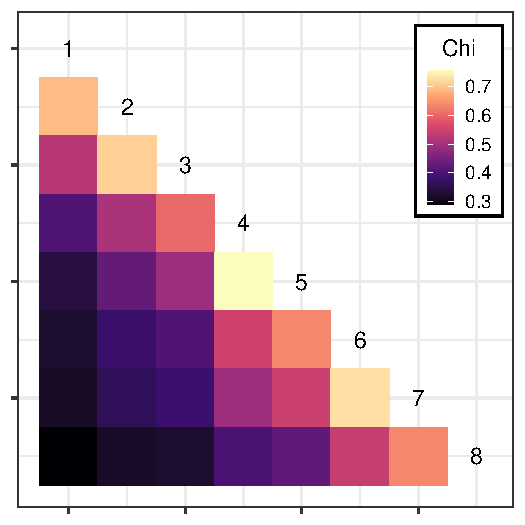
\includegraphics[width=0.99\linewidth]{./images/chi_ij_8}
    \end{minipage}
    \begin{minipage}{.49\textwidth}
      \centering
      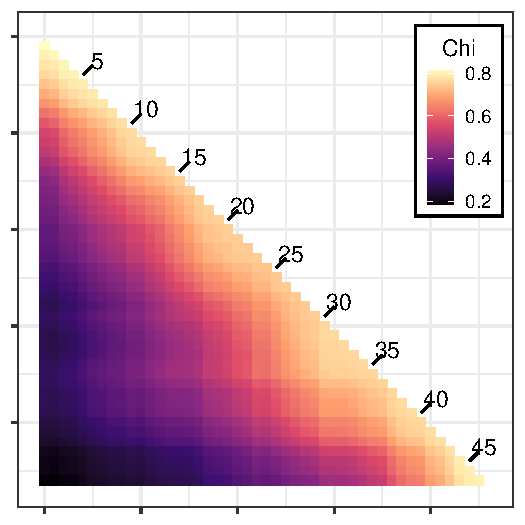
\includegraphics[width=0.99\linewidth]{./images/chi_ij_46}
    \end{minipage}
  \end{figure}

Figure~\ref{fig:chi_ij} plots the pairwise extremal dependence coefficients for the IVT data, in 8
  cells (left) and 47 cells (right), computed fom a fitted DP mixture of projected restricted gammas.
  We see a higher extremal dependence between neighboring columns which is not unexpected, as
  neighboring columns correspond to neighboring cells.  We recognize that pairwise asymptotic
  dependence coefficients tell a limited story, as a particular dependence may structure may include
  more than two columns.   We can, however, glean some information from the patterns that emerge in
  two dimensions.  On the 8-cell data, we see a stronger association between cells 5-8, indicating a
  greater dependence among these cells.  On the 47 cell data, we see at least 3 groupings of columns,
  indicating greater asymptotic dependence among these groups.

\subsection{Conditional Survival Curves}
Another interesting inference we can make from a fitted model is a conditional survival curve.
  Following rules of conditional probability, we can develop survival curves based on
  threshold exceedences. For ${\bf Z} = (Z_1,\ldots,Z_d)$ following a $d$-variate Pareto
  distribution, we make the proposition:

\begin{prop}
    In one dimension, the conditional survival curve can be calculated as
 \begin{equation}
    \label{eqn:condsurv1df}
    \text{P}\left[Z_{\ell} > z_{\ell}\mid {\bf Z}_{\neg(\ell)} > {\bf z}_{\neg(\ell)}\right] =
      \frac{\text{E}\left[\wedge_{k = 1}^d \frac{V_k}{z_k}\right]}{\text{E}\left[\bigwedge_{k \neq l}\frac{V_k}{z_k}\right]}
  \end{equation}
    where $\bm{V} = \bm{Z} / \pnorm{\bm{Z}}{\infty}$.
\end{prop}

By simple application of conditional probability, we expand the conditional survival function into
  a ratio of probabilities:
  \begin{equation}
    \label{eqn:condsurv1d}
    \text{P}\left[Z_{\ell} > z_{\ell}\mid {\bf Z}_{\neg(\ell)} > {\bf z}_{\neg(\ell)}\right] =
      \frac{\text{P}\left[\cap_{k = 1}^d Z_k > z_k\right]}{\text{P}\left[\cap_{k \neq l} Z_k > z_k\right]}.
  \end{equation}
  Let $R = \pnorm{{\bf Z}}{\infty}$, ${\bf V} = \frac{{\bf Z}}{R}$, such that ${\bf V}\in \mathcal{S}_{\infty}^{d-1}$.
  For evaluating these probabilities, recall that ${\bf Z} = R{\bf V}$.  Then,
  \begin{equation}
    \text{P}\left(\cap_{k = 1}^d Z_k > z_k\right) = \text{P}\left(\cap_{k = 1}^d RV_k > z_k\right)
  \end{equation}
  Also, for standard Pareto, recall that $\text{P}(R > r) = 1\wedge\frac{1}{r}$.  Then,
  \begin{equation}
    \text{P}\left[\bigcap_{k = 1}^d R > \frac{z_k}{V_k}\right] =
      \text{P}\left[R  > \bigvee_{k=1}^d\frac{z_k}{V_k}\right] =
      \text{E}\left[1 \bigwedge \left(\bigvee_{k = 1}^d\frac{z_k}{V_k}\right)^{-1}\right].
  \end{equation}
  As $V_k \in [0,1]$, and given our interest in the tail of the distribution, we can assume
  $z_k > 1$, therefore $\frac{z_k}{V_k} > 1$.  We thus arrive at
  \begin{equation}
    \text{P}\left[\cap_{k = 1}^d Z_k > z_k\right] = \text{E}\left[\wedge_{k = 1}^d\frac{V_i}{z_i}\right].
  \end{equation}
  We employ a similar calculation in the denominator, yielding
  \begin{equation}
    \text{P}\left[Z_{\ell} > z_{\ell}\mid {\bf Z}_{\neg(l)} > {\bf z}_{\neg(l)}\right] =
      \frac{\text{E}\left[\wedge_{k = 1}^d \frac{V_k}{z_k}\right]}{\text{E}\left[\bigwedge_{k \neq \ell}\frac{V_k}{z_k}\right]}
  \end{equation}
  Figure~\ref{fig:condsurv1d} displays this conditional survival function for the 8 cell data. For each
  cell, the survival function is computed given all other cells are at or above their $90$th marginal
  percentile.

\begin{figure}[b]
  \caption{
    Single-variable conditional survival function in extreme
    regions---$\text{Pr}[Z_{\ell} > z_{\ell}\mid Z_{\neg l} > z_{\neg l}]$,
    evaluated where $z_{\neg l} = F_{\neg l}^{-1}(0.9)$---for the 8-cell data.  The model used to
    generate this estimate is the DP mixture of projected restricted Gammas.\label{fig:condsurv1d}
    }
  \centering
  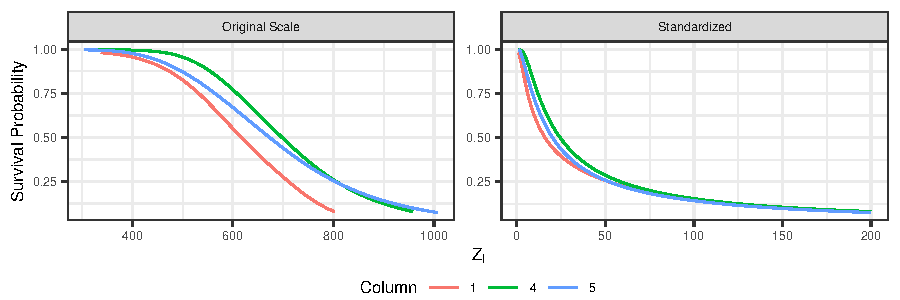
\includegraphics[width = 5in]{./images/condsurv_1d}
\end{figure}

Following similar calculations, for a dimension set $\alpha \subset \{1,\ldots, d\}$, a multivariate
  conditional survival function can be similarly estimated as
  \begin{equation}
    \label{eqn:condsurv2df}
    \text{P}\left[\bigcap_{\ell \in \alpha} Z_{\ell} > z_{\ell} \mid \bigcap_{\ell\not\in\alpha} Z_{\ell} > z_{\ell}\right] =
      \frac{\text{E}\left[\bigwedge_{k = 1}^d \frac{V_k}{z_k}\right]}{\text{E}\left[\bigwedge_{k \not\in\alpha}\frac{V_k}{z_k}\right]}.
  \end{equation}
  Figure~\ref{fig:condsurv2d} displays selected bi-variate conditional survival surfaces, for the 8-cell
  data.  For each pair of cells, the survival function is again computed conditional on  all other cells
  at or above their $90$th percentile.  Note, for cell pairs (1,2) and (7,8), the strong asymptotic dependence
  observed in Figure~\ref{fig:chi_ij} exhibits itself in a greater tendency towards jointly extreme
  behavior in the survival function; whereas cell pairs (1,6) and (2,8) show their low asymptotic
  dependence with a low propensity towards jointly extreme behavior.

\begin{figure}[t]
  \caption{
    Selected bi-variate conditional survival surfaces in extreme regions for the 8 cell data.
    The DP mixture of projected restricted Gammas model was used to generate these surfaces.
    \label{fig:condsurv2d}
    }
  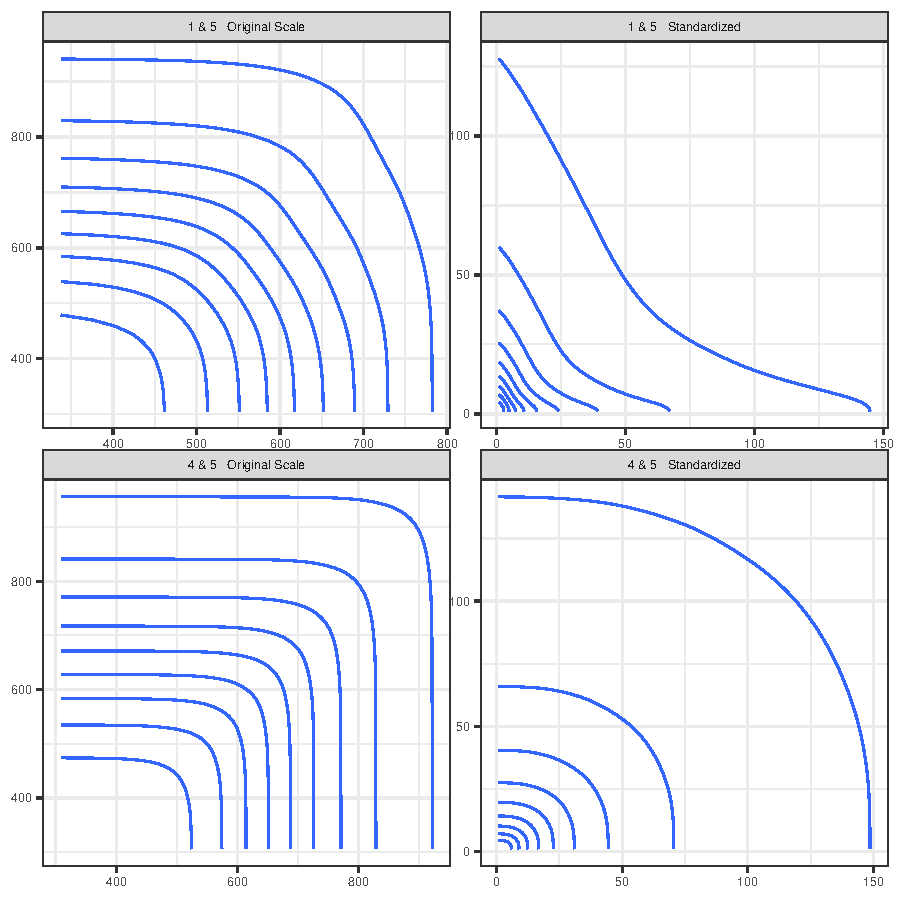
\includegraphics{./images/condsurv_2d}
\end{figure}










% EOF
